\documentclass[../main.tex]{subfiles}

\begin{document}

One of the key innovations of this algorithm is that it performs efficient vector searches using vector compression techniques. The aim of this section is to assess the effectiveness of such compression and evaluate its influence on the quality of the results.

Several compression techniques will be considered in order to select the best compromise between speed and accuracy. Similarly to the previous experiments, the tests will be carried out with a resolution limit of $15 \si{\angstrom}$. For reference, an alignment without any vector compression will also be considered. The raw input vectors have on average around $1300$ components, which require $5200 \si{\byte}$ to be stored in 32 bit floating point format.

The first evaluated compression technique will be a \gls{pca}. As stated in Chapter \ref{chap:implementation}, this compression technique reduces the dimensionality though a linear projection in such a way that most of the signal energy is kept. In this case, input vectors will be reduced to $128$ and $64$ components, leading to an approximate compression rate of x10 and x20, respectively. These vectors will have a constant storage cost of $512\si{\byte}$ and $256\si{\byte}$. Additionally the \gls{pca} projection matrix needs to be stored, which has a inappreciable size when a large quantity of vectors is used.

Secondly, the \gls{ivf}-\gls{pq} vector compression technique described in Chapter \ref{chap:implementation} will be tested. In this case, each block of the vector will be quantised into 256 cells, so that a single byte can be used to represent it. The vector will be divided either in 48 or 32 blocks, so that $48\si{\byte}$ or $32\si{\byte}$ are needed to store it. In this case, the compression ratios are in the order of x100.

The Figure \ref{fig:5:vector_size} illustrates the storage costs for each of the vector compression techniques. Compressed vectors have a size that is agnostic of the dataset. However, the size of the raw vector depends on the image size and its sampling rate. Therefore, the plot shows bars for each of the datasets, although only the first bar varies across acquisitions. Note that the vertical axis of the graph is logarithmic, suggesting that there is an order of magnitude of difference between not using any compression, using \gls{pca} compression and using \gls{ivf}-\gls{pq} compression.

\begin{figure}[htbp]
    \centering
    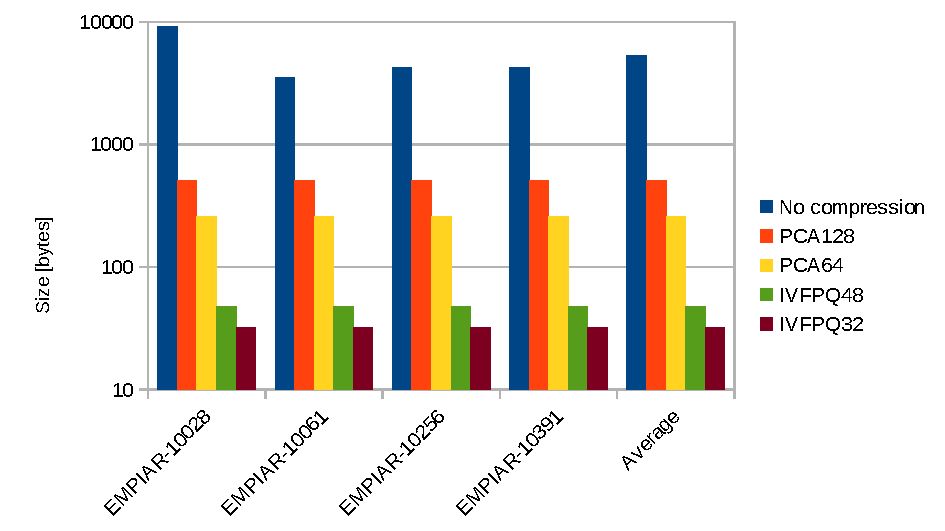
\includegraphics[width=.8\textwidth]{results/compression/vector size}
    \caption{Vector storage size comparison between vector compression techniques}
    \label{fig:5:vector_size}
\end{figure}

\subsubsection{Accuracy}
Regarding the empirical results, we have been able to measure some degree of accuracy degradation directly related to vector compression. In general, there is correlation between the accuracy loss and the compression ratio employed for storing the vectors. However, the relation is not linear, as the compression ratio raises by orders of magnitude while the decrease in precision is slight. Moreover, the performance increase is considerable.

Figures \ref{fig:5:compression_angle_accuracy} and \ref{fig:5:compression_shift_accuracy} point out that in the case of experimental images, the this degradation is considerably lesser. On average the results of \gls{pca}-64 compression are worse than the results of of \gls{ivf}-\gls{pq} compression techniques, which offers a higher compression ratio. In any case, results with simulated images have a more pronounced influence of the compression. Once again, the bad results obtained with EMPIAR-10256 make the average results very bad. 

\begin{figure}[htbp]
    \centering
    \begin{subfigure}[b]{.8\textwidth}
         \centering
         \includegraphics[width=\linewidth]{results/compression/simulated/angle error}
         \caption{Simulated images}
    \end{subfigure}\\
    \vspace{2em}
    \begin{subfigure}[b]{.8\textwidth}
         \centering
         \includegraphics[width=\linewidth]{results/compression/experimental/angle error}
         \caption{Experimental images}
    \end{subfigure}
    \caption{Angle accuracy for different vector compression methods}
    \label{fig:5:compression_angle_accuracy}
\end{figure}

\begin{figure}[htbp]
    \centering
    \begin{subfigure}[b]{.8\textwidth}
         \centering
         \includegraphics[width=\linewidth]{results/compression/simulated/shift error}
         \caption{Simulated images}
    \end{subfigure}\\
    \vspace{2em}
    \begin{subfigure}[b]{.8\textwidth}
         \centering
         \includegraphics[width=\linewidth]{results/compression/experimental/shift error}
         \caption{Experimental images}
    \end{subfigure}
    \caption{Shift accuracy for different vector compression methods}
    \label{fig:5:compression_shift_accuracy}
\end{figure}

When employing these particles to reconstruct a new volume, the resolutions obtained are shown in Figure \ref{fig:5:compression_resolution}. It can be observed that simulated images produce similar reconstruction resolutions, regardless of the compression method used, but accuracy significantly varies across compression methods. This suggests that the alignment errors of these datasets are induced by very similar views of the volume, as the reconstruction resolution is not affected. Concerning the experimental images, the alignment errors measured earlier correlate with lower reconstruction resolutions.

\begin{figure}[htbp]
    \centering
    \begin{subfigure}[b]{.8\textwidth}
         \centering
         \includegraphics[width=\linewidth]{results/compression/simulated/resolution}
         \caption{Simulated images}
    \end{subfigure}\\
    \vspace{2em}
    \begin{subfigure}[b]{.8\textwidth}
         \centering
         \includegraphics[width=\linewidth]{results/compression/experimental/resolution}
         \caption{Experimental images}
    \end{subfigure}
    \caption{Reconstruction resolution for different vector compression methods}
    \label{fig:5:compression_resolution}
\end{figure}

\subsubsection{Performance}
The compression ratio is also highly correlated with the alignment time. Higher compression ratios involve faster memory access times and also quicker distance computations. Thus, the alignment times with vector compression are considerably faster. In this analysis we have distinguished two parts regarding the alignment times. The first one is related to the constant part, which is related to the database training and population processes. This time remains invariant regardless of the number of particles to be aligned. The second part is the time spent on the alignment process itself. This time scales linearly with the number of particles, thus, its measurement is provided as the time per particle (the slope of the linear relationship).

Figure \ref{fig:5:compression_constant} proves that the training process required for compression is amortized from the first particle, since the saved time in populating the database compensates this additional step. In any case, the differences in time related to different compression techniques are very subtle. When aligning reasonable amounts of particles, these differences are negligible.

\begin{figure}[htbp]
    \centering
    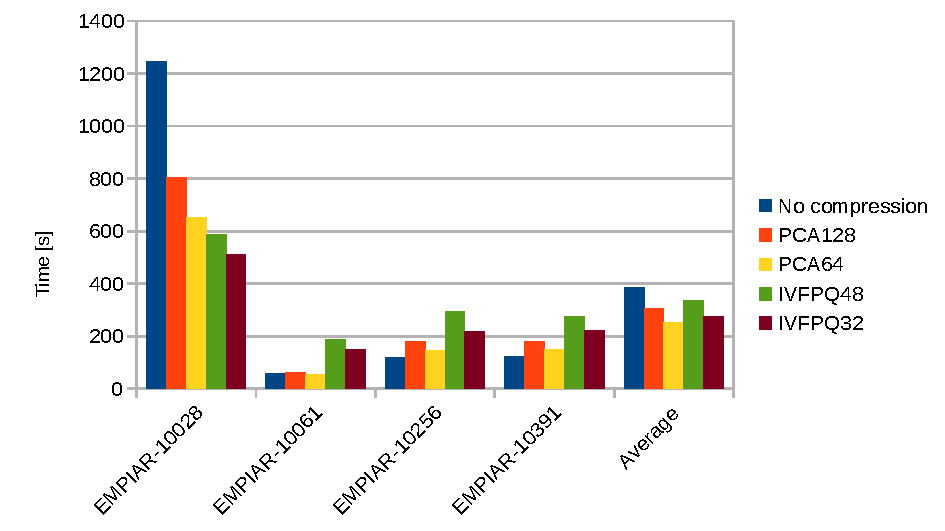
\includegraphics[width=.8\linewidth]{results/compression/simulated/const time}
    \caption{Constant time (Training + Populate) for different vector compression methods}
    \label{fig:5:compression_constant}
\end{figure}

The time required to align individual particles is represented in Figure \ref{fig:5:compression_alignment}, which can be interpreted as the slope of the function representing the total alignment time in terms of the particle count. It is important to note that this graph has vertical logarithmic spacing. Consequently, even slight variations in the graph can result in significant time savings. Considering the significance of this factor for datasets of practical sizes, these numbers serve as the basis for drawing conclusions regarding vector compression techniques.

\begin{figure}[htbp]
    \centering
    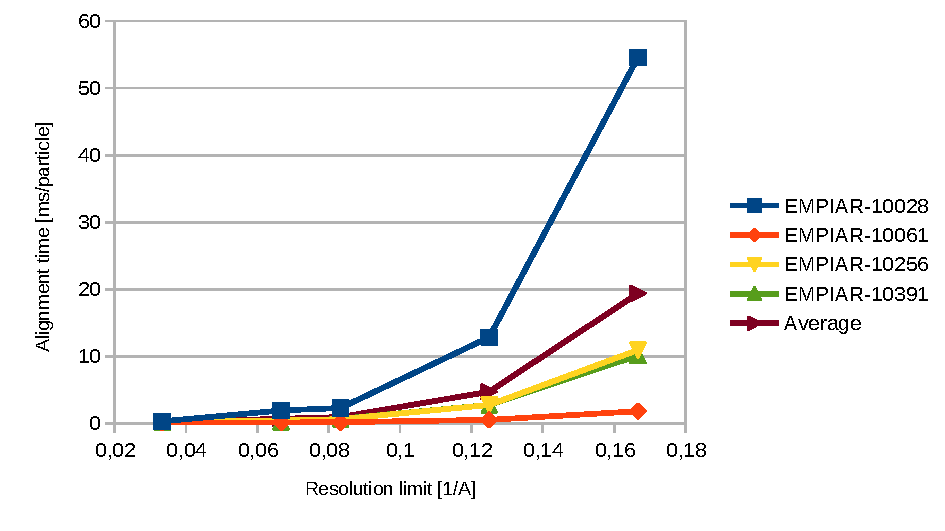
\includegraphics[width=.8\linewidth]{results/compression/simulated/alignment time}
    \caption{Alignment time for different vector compression methods}
    \label{fig:5:compression_alignment}
\end{figure}

On average, the usage on any compression method significantly reduces the alignment time. This is specially true for \gls{ivf}-\gls{pq} technique, which obtains a x10 speedup in comparison to the uncompressed vectors. Indeed there is no speedup when varying the number of bytes used with \gls{ivf}-\gls{pq}, so the 48B version should be preferred, as it offers better accuracy results. Similarly, \gls{pca}64 provides similar accuracy results but it is slower. As a consequence, \gls{pca}64 and \gls{ivf}-\gls{pq}32 compression techniques can be safely dismissed. At the end we have chosen to use the \gls{ivf}-\gls{pq}48 technique, as it is more than twice as fast as the \gls{pca}128 option at a slight accuracy cost. Later we will explore options to trade back this performance gain with better accuracy results.

\end{document}